% Created by tikzDevice version 0.12.6 on 2026-07-03 11:54:53
% !TEX encoding = UTF-8 Unicode
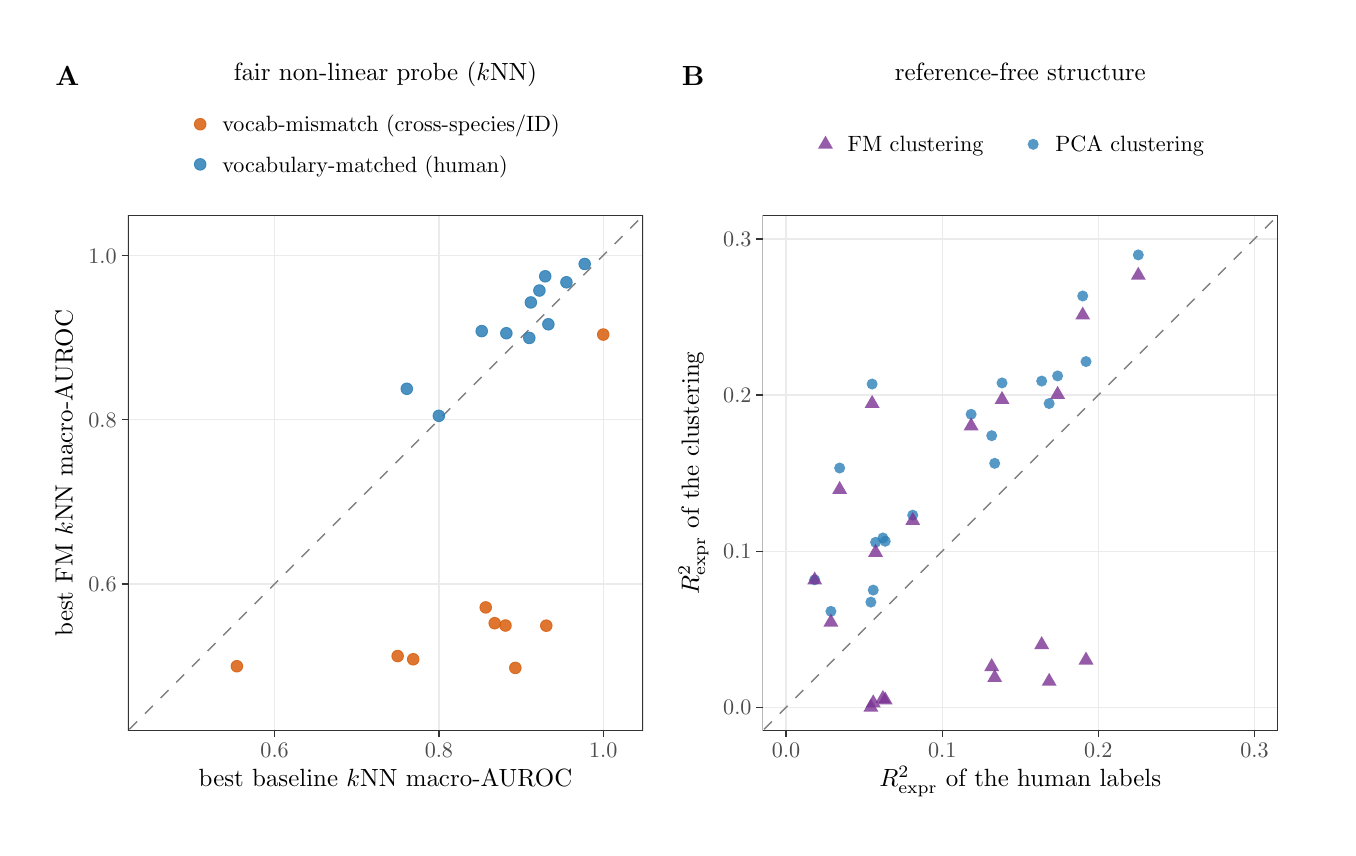
\begin{tikzpicture}[x=1pt,y=1pt]
\definecolor{fillColor}{RGB}{255,255,255}
\path[use as bounding box,fill=fillColor,fill opacity=0.00] (0,0) rectangle (469.75,289.08);
\begin{scope}
\path[clip] (  0.00,  2.95) rectangle (469.75,286.13);
\definecolor{drawColor}{RGB}{255,255,255}
\definecolor{fillColor}{RGB}{255,255,255}

\path[draw=drawColor,line width= 0.5pt,line join=round,line cap=round,fill=fillColor] (  0.00,  2.95) rectangle (469.75,286.13);
\end{scope}
\begin{scope}
\path[clip] (  5.00,  7.95) rectangle (231.38,281.13);
\definecolor{drawColor}{RGB}{255,255,255}
\definecolor{fillColor}{RGB}{255,255,255}

\path[draw=drawColor,line width= 0.5pt,line join=round,line cap=round,fill=fillColor] (  5.00,  7.95) rectangle (231.38,281.13);
\end{scope}
\begin{scope}
\path[clip] (231.38,  7.95) rectangle (460.75,281.13);
\definecolor{drawColor}{RGB}{255,255,255}
\definecolor{fillColor}{RGB}{255,255,255}

\path[draw=drawColor,line width= 0.5pt,line join=round,line cap=round,fill=fillColor] (231.38,  7.95) rectangle (460.75,281.13);
\end{scope}
\begin{scope}
\path[clip] ( 36.22, 35.02) rectangle (222.38,221.18);
\definecolor{fillColor}{RGB}{255,255,255}

\path[fill=fillColor] ( 36.22, 35.02) rectangle (222.38,221.18);
\definecolor{drawColor}{gray}{0.92}

\path[draw=drawColor,line width= 0.5pt,line join=round] ( 36.22, 88.02) --
	(222.38, 88.02);

\path[draw=drawColor,line width= 0.5pt,line join=round] ( 36.22,147.40) --
	(222.38,147.40);

\path[draw=drawColor,line width= 0.5pt,line join=round] ( 36.22,206.78) --
	(222.38,206.78);

\path[draw=drawColor,line width= 0.5pt,line join=round] ( 89.22, 35.02) --
	( 89.22,221.18);

\path[draw=drawColor,line width= 0.5pt,line join=round] (148.60, 35.02) --
	(148.60,221.18);

\path[draw=drawColor,line width= 0.5pt,line join=round] (207.98, 35.02) --
	(207.98,221.18);
\definecolor{drawColor}{gray}{0.50}

\path[draw=drawColor,line width= 0.5pt,dash pattern=on 4pt off 4pt ,line join=round] (-149.93,-151.13) -- (408.53,407.33);
\definecolor{drawColor}{RGB}{44,127,184}
\definecolor{fillColor}{RGB}{44,127,184}

\path[draw=drawColor,draw opacity=0.85,line width= 0.3pt,line join=round,line cap=round,fill=fillColor,fill opacity=0.85] (184.91,194.10) circle (  2.11);

\path[draw=drawColor,draw opacity=0.85,line width= 0.3pt,line join=round,line cap=round,fill=fillColor,fill opacity=0.85] (136.99,158.59) circle (  2.11);
\definecolor{drawColor}{RGB}{217,95,14}
\definecolor{fillColor}{RGB}{217,95,14}

\path[draw=drawColor,draw opacity=0.85,line width= 0.3pt,line join=round,line cap=round,fill=fillColor,fill opacity=0.85] (172.65, 73.05) circle (  2.11);
\definecolor{drawColor}{RGB}{44,127,184}
\definecolor{fillColor}{RGB}{44,127,184}

\path[draw=drawColor,draw opacity=0.85,line width= 0.3pt,line join=round,line cap=round,fill=fillColor,fill opacity=0.85] (148.57,148.82) circle (  2.11);

\path[draw=drawColor,draw opacity=0.85,line width= 0.3pt,line join=round,line cap=round,fill=fillColor,fill opacity=0.85] (172.97,178.66) circle (  2.11);
\definecolor{drawColor}{RGB}{217,95,14}
\definecolor{fillColor}{RGB}{217,95,14}

\path[draw=drawColor,draw opacity=0.85,line width= 0.3pt,line join=round,line cap=round,fill=fillColor,fill opacity=0.85] (165.52, 79.59) circle (  2.11);
\definecolor{drawColor}{RGB}{44,127,184}
\definecolor{fillColor}{RGB}{44,127,184}

\path[draw=drawColor,draw opacity=0.85,line width= 0.3pt,line join=round,line cap=round,fill=fillColor,fill opacity=0.85] (181.26,176.97) circle (  2.11);
\definecolor{drawColor}{RGB}{217,95,14}
\definecolor{fillColor}{RGB}{217,95,14}

\path[draw=drawColor,draw opacity=0.85,line width= 0.3pt,line join=round,line cap=round,fill=fillColor,fill opacity=0.85] (168.76, 73.88) circle (  2.11);
\definecolor{drawColor}{RGB}{44,127,184}
\definecolor{fillColor}{RGB}{44,127,184}

\path[draw=drawColor,draw opacity=0.85,line width= 0.3pt,line join=round,line cap=round,fill=fillColor,fill opacity=0.85] (188.15,181.90) circle (  2.11);

\path[draw=drawColor,draw opacity=0.85,line width= 0.3pt,line join=round,line cap=round,fill=fillColor,fill opacity=0.85] (164.07,179.43) circle (  2.11);

\path[draw=drawColor,draw opacity=0.85,line width= 0.3pt,line join=round,line cap=round,fill=fillColor,fill opacity=0.85] (194.68,197.07) circle (  2.11);

\path[draw=drawColor,draw opacity=0.85,line width= 0.3pt,line join=round,line cap=round,fill=fillColor,fill opacity=0.85] (181.82,189.79) circle (  2.11);
\definecolor{drawColor}{RGB}{217,95,14}
\definecolor{fillColor}{RGB}{217,95,14}

\path[draw=drawColor,draw opacity=0.85,line width= 0.3pt,line join=round,line cap=round,fill=fillColor,fill opacity=0.85] (207.98,178.19) circle (  2.11);

\path[draw=drawColor,draw opacity=0.85,line width= 0.3pt,line join=round,line cap=round,fill=fillColor,fill opacity=0.85] ( 75.59, 58.33) circle (  2.11);

\path[draw=drawColor,draw opacity=0.85,line width= 0.3pt,line join=round,line cap=round,fill=fillColor,fill opacity=0.85] (176.21, 57.73) circle (  2.11);
\definecolor{drawColor}{RGB}{44,127,184}
\definecolor{fillColor}{RGB}{44,127,184}

\path[draw=drawColor,draw opacity=0.85,line width= 0.3pt,line join=round,line cap=round,fill=fillColor,fill opacity=0.85] (201.27,203.69) circle (  2.11);
\definecolor{drawColor}{RGB}{217,95,14}
\definecolor{fillColor}{RGB}{217,95,14}

\path[draw=drawColor,draw opacity=0.85,line width= 0.3pt,line join=round,line cap=round,fill=fillColor,fill opacity=0.85] (133.69, 62.01) circle (  2.11);
\definecolor{drawColor}{RGB}{44,127,184}
\definecolor{fillColor}{RGB}{44,127,184}

\path[draw=drawColor,draw opacity=0.85,line width= 0.3pt,line join=round,line cap=round,fill=fillColor,fill opacity=0.85] (187.02,199.24) circle (  2.11);
\definecolor{drawColor}{RGB}{217,95,14}
\definecolor{fillColor}{RGB}{217,95,14}

\path[draw=drawColor,draw opacity=0.85,line width= 0.3pt,line join=round,line cap=round,fill=fillColor,fill opacity=0.85] (187.40, 72.99) circle (  2.11);

\path[draw=drawColor,draw opacity=0.85,line width= 0.3pt,line join=round,line cap=round,fill=fillColor,fill opacity=0.85] (139.31, 60.85) circle (  2.11);
\definecolor{drawColor}{gray}{0.20}

\path[draw=drawColor,line width= 0.5pt,line join=round,line cap=round] ( 36.22, 35.02) rectangle (222.38,221.18);
\end{scope}
\begin{scope}
\path[clip] (  0.00,  0.00) rectangle (469.75,289.08);
\definecolor{drawColor}{gray}{0.30}

\node[text=drawColor,anchor=base east,inner sep=0pt, outer sep=0pt, scale=  0.80] at ( 32.17, 85.26) {0.6};

\node[text=drawColor,anchor=base east,inner sep=0pt, outer sep=0pt, scale=  0.80] at ( 32.17,144.64) {0.8};

\node[text=drawColor,anchor=base east,inner sep=0pt, outer sep=0pt, scale=  0.80] at ( 32.17,204.02) {1.0};
\end{scope}
\begin{scope}
\path[clip] (  0.00,  0.00) rectangle (469.75,289.08);
\definecolor{drawColor}{gray}{0.20}

\path[draw=drawColor,line width= 0.5pt,line join=round] ( 33.97, 88.02) --
	( 36.22, 88.02);

\path[draw=drawColor,line width= 0.5pt,line join=round] ( 33.97,147.40) --
	( 36.22,147.40);

\path[draw=drawColor,line width= 0.5pt,line join=round] ( 33.97,206.78) --
	( 36.22,206.78);
\end{scope}
\begin{scope}
\path[clip] (  0.00,  0.00) rectangle (469.75,289.08);
\definecolor{drawColor}{RGB}{0,0,0}

\node[text=drawColor,rotate= 90.00,anchor=base,inner sep=0pt, outer sep=0pt, scale=  0.90] at ( 16.20,128.10) {best FM $k$NN macro-AUROC};
\end{scope}
\begin{scope}
\path[clip] (  0.00,  0.00) rectangle (469.75,289.08);
\definecolor{drawColor}{gray}{0.20}

\path[draw=drawColor,line width= 0.5pt,line join=round] ( 89.22, 32.77) --
	( 89.22, 35.02);

\path[draw=drawColor,line width= 0.5pt,line join=round] (148.60, 32.77) --
	(148.60, 35.02);

\path[draw=drawColor,line width= 0.5pt,line join=round] (207.98, 32.77) --
	(207.98, 35.02);
\end{scope}
\begin{scope}
\path[clip] (  0.00,  0.00) rectangle (469.75,289.08);
\definecolor{drawColor}{gray}{0.30}

\node[text=drawColor,anchor=base,inner sep=0pt, outer sep=0pt, scale=  0.80] at ( 89.22, 25.46) {0.6};

\node[text=drawColor,anchor=base,inner sep=0pt, outer sep=0pt, scale=  0.80] at (148.60, 25.46) {0.8};

\node[text=drawColor,anchor=base,inner sep=0pt, outer sep=0pt, scale=  0.80] at (207.98, 25.46) {1.0};
\end{scope}
\begin{scope}
\path[clip] (  0.00,  0.00) rectangle (469.75,289.08);
\definecolor{drawColor}{RGB}{0,0,0}

\node[text=drawColor,anchor=base,inner sep=0pt, outer sep=0pt, scale=  0.90] at (129.30, 14.70) {best baseline $k$NN macro-AUROC};
\end{scope}
\begin{scope}
\path[clip] (  0.00,  0.00) rectangle (469.75,289.08);
\definecolor{fillColor}{RGB}{255,255,255}

\path[fill=fillColor] ( 52.84,230.18) rectangle (205.76,263.68);
\end{scope}
\begin{scope}
\path[clip] (  0.00,  0.00) rectangle (469.75,289.08);
\definecolor{fillColor}{RGB}{255,255,255}

\path[fill=fillColor] ( 57.34,249.18) rectangle ( 67.34,259.18);
\definecolor{drawColor}{RGB}{217,95,14}
\definecolor{fillColor}{RGB}{217,95,14}

\path[draw=drawColor,draw opacity=0.85,line width= 0.3pt,line join=round,line cap=round,fill=fillColor,fill opacity=0.85] ( 62.34,254.18) circle (  2.11);
\end{scope}
\begin{scope}
\path[clip] (  0.00,  0.00) rectangle (469.75,289.08);
\definecolor{fillColor}{RGB}{255,255,255}

\path[fill=fillColor] ( 57.34,234.68) rectangle ( 67.34,244.68);
\definecolor{drawColor}{RGB}{44,127,184}
\definecolor{fillColor}{RGB}{44,127,184}

\path[draw=drawColor,draw opacity=0.85,line width= 0.3pt,line join=round,line cap=round,fill=fillColor,fill opacity=0.85] ( 62.34,239.68) circle (  2.11);
\end{scope}
\begin{scope}
\path[clip] (  0.00,  0.00) rectangle (469.75,289.08);
\definecolor{drawColor}{RGB}{0,0,0}

\node[text=drawColor,anchor=base west,inner sep=0pt, outer sep=0pt, scale=  0.80] at ( 70.34,251.42) {vocab-mismatch (cross-species/ID)};
\end{scope}
\begin{scope}
\path[clip] (  0.00,  0.00) rectangle (469.75,289.08);
\definecolor{drawColor}{RGB}{0,0,0}

\node[text=drawColor,anchor=base west,inner sep=0pt, outer sep=0pt, scale=  0.80] at ( 70.34,236.92) {vocabulary-matched (human)};
\end{scope}
\begin{scope}
\path[clip] (  0.00,  0.00) rectangle (469.75,289.08);
\definecolor{drawColor}{RGB}{0,0,0}

\node[text=drawColor,anchor=base,inner sep=0pt, outer sep=0pt, scale=  0.90] at (129.30,269.93) {fair non-linear probe ($k$NN)};
\end{scope}
\begin{scope}
\path[clip] (  0.00,  0.00) rectangle (469.75,289.08);
\definecolor{drawColor}{RGB}{0,0,0}

\node[text=drawColor,anchor=base,inner sep=0pt, outer sep=0pt, scale=  1.00] at ( 14.35,268.16) {\bfseries A};
\end{scope}
\begin{scope}
\path[clip] (265.60, 35.02) rectangle (451.75,221.18);
\definecolor{fillColor}{RGB}{255,255,255}

\path[fill=fillColor] (265.60, 35.02) rectangle (451.75,221.18);
\definecolor{drawColor}{gray}{0.92}

\path[draw=drawColor,line width= 0.5pt,line join=round] (265.60, 43.48) --
	(451.75, 43.48);

\path[draw=drawColor,line width= 0.5pt,line join=round] (265.60, 99.89) --
	(451.75, 99.89);

\path[draw=drawColor,line width= 0.5pt,line join=round] (265.60,156.30) --
	(451.75,156.30);

\path[draw=drawColor,line width= 0.5pt,line join=round] (265.60,212.71) --
	(451.75,212.71);

\path[draw=drawColor,line width= 0.5pt,line join=round] (274.06, 35.02) --
	(274.06,221.18);

\path[draw=drawColor,line width= 0.5pt,line join=round] (330.47, 35.02) --
	(330.47,221.18);

\path[draw=drawColor,line width= 0.5pt,line join=round] (386.88, 35.02) --
	(386.88,221.18);

\path[draw=drawColor,line width= 0.5pt,line join=round] (443.29, 35.02) --
	(443.29,221.18);
\definecolor{drawColor}{gray}{0.50}

\path[draw=drawColor,line width= 0.5pt,dash pattern=on 4pt off 4pt ,line join=round] ( 79.44,-151.13) -- (637.91,407.33);
\definecolor{fillColor}{RGB}{44,127,184}

\path[fill=fillColor,fill opacity=0.80] (319.81,112.92) circle (  2.00);

\path[fill=fillColor,fill opacity=0.80] (306.38,103.11) circle (  2.00);

\path[fill=fillColor,fill opacity=0.80] (349.43,131.65) circle (  2.00);

\path[fill=fillColor,fill opacity=0.80] (401.32,206.96) circle (  2.00);

\path[fill=fillColor,fill opacity=0.80] (290.25, 78.17) circle (  2.00);

\path[fill=fillColor,fill opacity=0.80] (366.41,161.38) circle (  2.00);

\path[fill=fillColor,fill opacity=0.80] (340.91,149.37) circle (  2.00);

\path[fill=fillColor,fill opacity=0.80] (382.43,168.43) circle (  2.00);

\path[fill=fillColor,fill opacity=0.80] (305.14,160.31) circle (  2.00);

\path[fill=fillColor,fill opacity=0.80] (284.38, 89.57) circle (  2.00);

\path[fill=fillColor,fill opacity=0.80] (381.24,192.12) circle (  2.00);

\path[fill=fillColor,fill opacity=0.80] (372.16,163.24) circle (  2.00);

\path[fill=fillColor,fill opacity=0.80] (369.11,153.26) circle (  2.00);

\path[fill=fillColor,fill opacity=0.80] (304.69, 81.50) circle (  2.00);

\path[fill=fillColor,fill opacity=0.80] (305.54, 85.85) circle (  2.00);

\path[fill=fillColor,fill opacity=0.80] (352.08,160.70) circle (  2.00);

\path[fill=fillColor,fill opacity=0.80] (309.88,103.50) circle (  2.00);

\path[fill=fillColor,fill opacity=0.80] (293.41,129.96) circle (  2.00);

\path[fill=fillColor,fill opacity=0.80] (348.35,141.64) circle (  2.00);

\path[fill=fillColor,fill opacity=0.80] (309.04,104.69) circle (  2.00);
\definecolor{fillColor}{RGB}{123,50,148}

\path[fill=fillColor,fill opacity=0.80] (319.81,114.07) --
	(322.51,109.39) --
	(317.11,109.39) --
	cycle;

\path[fill=fillColor,fill opacity=0.80] (306.38,102.56) --
	(309.08, 97.88) --
	(303.68, 97.88) --
	cycle;

\path[fill=fillColor,fill opacity=0.80] (349.43, 57.32) --
	(352.13, 52.64) --
	(346.73, 52.64) --
	cycle;

\path[fill=fillColor,fill opacity=0.80] (401.32,202.69) --
	(404.02,198.01) --
	(398.62,198.01) --
	cycle;

\path[fill=fillColor,fill opacity=0.80] (290.25, 77.34) --
	(292.95, 72.67) --
	(287.55, 72.67) --
	cycle;

\path[fill=fillColor,fill opacity=0.80] (366.41, 69.22) --
	(369.11, 64.54) --
	(363.71, 64.54) --
	cycle;

\path[fill=fillColor,fill opacity=0.80] (340.91,148.25) --
	(343.61,143.58) --
	(338.21,143.58) --
	cycle;

\path[fill=fillColor,fill opacity=0.80] (382.43, 63.64) --
	(385.13, 58.96) --
	(379.73, 58.96) --
	cycle;

\path[fill=fillColor,fill opacity=0.80] (305.14,156.37) --
	(307.84,151.70) --
	(302.44,151.70) --
	cycle;

\path[fill=fillColor,fill opacity=0.80] (284.38, 92.57) --
	(287.08, 87.90) --
	(281.68, 87.90) --
	cycle;

\path[fill=fillColor,fill opacity=0.80] (381.24,188.30) --
	(383.94,183.63) --
	(378.54,183.63) --
	cycle;

\path[fill=fillColor,fill opacity=0.80] (372.16,159.65) --
	(374.86,154.97) --
	(369.46,154.97) --
	cycle;

\path[fill=fillColor,fill opacity=0.80] (369.11, 55.96) --
	(371.81, 51.29) --
	(366.41, 51.29) --
	cycle;

\path[fill=fillColor,fill opacity=0.80] (304.69, 46.60) --
	(307.39, 41.92) --
	(301.99, 41.92) --
	cycle;

\path[fill=fillColor,fill opacity=0.80] (305.54, 48.18) --
	(308.24, 43.50) --
	(302.84, 43.50) --
	cycle;

\path[fill=fillColor,fill opacity=0.80] (352.08,157.79) --
	(354.78,153.11) --
	(349.38,153.11) --
	cycle;

\path[fill=fillColor,fill opacity=0.80] (309.88, 49.19) --
	(312.58, 44.52) --
	(307.18, 44.52) --
	cycle;

\path[fill=fillColor,fill opacity=0.80] (293.41,125.29) --
	(296.11,120.62) --
	(290.71,120.62) --
	cycle;

\path[fill=fillColor,fill opacity=0.80] (348.35, 61.27) --
	(351.05, 56.59) --
	(345.65, 56.59) --
	cycle;

\path[fill=fillColor,fill opacity=0.80] (309.04, 49.76) --
	(311.74, 45.08) --
	(306.34, 45.08) --
	cycle;
\definecolor{drawColor}{gray}{0.20}

\path[draw=drawColor,line width= 0.5pt,line join=round,line cap=round] (265.60, 35.02) rectangle (451.75,221.18);
\end{scope}
\begin{scope}
\path[clip] (  0.00,  0.00) rectangle (469.75,289.08);
\definecolor{drawColor}{gray}{0.30}

\node[text=drawColor,anchor=base east,inner sep=0pt, outer sep=0pt, scale=  0.80] at (261.55, 40.73) {0.0};

\node[text=drawColor,anchor=base east,inner sep=0pt, outer sep=0pt, scale=  0.80] at (261.55, 97.14) {0.1};

\node[text=drawColor,anchor=base east,inner sep=0pt, outer sep=0pt, scale=  0.80] at (261.55,153.55) {0.2};

\node[text=drawColor,anchor=base east,inner sep=0pt, outer sep=0pt, scale=  0.80] at (261.55,209.96) {0.3};
\end{scope}
\begin{scope}
\path[clip] (  0.00,  0.00) rectangle (469.75,289.08);
\definecolor{drawColor}{gray}{0.20}

\path[draw=drawColor,line width= 0.5pt,line join=round] (263.35, 43.48) --
	(265.60, 43.48);

\path[draw=drawColor,line width= 0.5pt,line join=round] (263.35, 99.89) --
	(265.60, 99.89);

\path[draw=drawColor,line width= 0.5pt,line join=round] (263.35,156.30) --
	(265.60,156.30);

\path[draw=drawColor,line width= 0.5pt,line join=round] (263.35,212.71) --
	(265.60,212.71);
\end{scope}
\begin{scope}
\path[clip] (  0.00,  0.00) rectangle (469.75,289.08);
\definecolor{drawColor}{RGB}{0,0,0}

\node[text=drawColor,rotate= 90.00,anchor=base,inner sep=0pt, outer sep=0pt, scale=  0.90] at (242.58,128.10) {$R^2_{\mathrm{expr}}$ of the clustering};
\end{scope}
\begin{scope}
\path[clip] (  0.00,  0.00) rectangle (469.75,289.08);
\definecolor{drawColor}{gray}{0.20}

\path[draw=drawColor,line width= 0.5pt,line join=round] (274.06, 32.77) --
	(274.06, 35.02);

\path[draw=drawColor,line width= 0.5pt,line join=round] (330.47, 32.77) --
	(330.47, 35.02);

\path[draw=drawColor,line width= 0.5pt,line join=round] (386.88, 32.77) --
	(386.88, 35.02);

\path[draw=drawColor,line width= 0.5pt,line join=round] (443.29, 32.77) --
	(443.29, 35.02);
\end{scope}
\begin{scope}
\path[clip] (  0.00,  0.00) rectangle (469.75,289.08);
\definecolor{drawColor}{gray}{0.30}

\node[text=drawColor,anchor=base,inner sep=0pt, outer sep=0pt, scale=  0.80] at (274.06, 25.46) {0.0};

\node[text=drawColor,anchor=base,inner sep=0pt, outer sep=0pt, scale=  0.80] at (330.47, 25.46) {0.1};

\node[text=drawColor,anchor=base,inner sep=0pt, outer sep=0pt, scale=  0.80] at (386.88, 25.46) {0.2};

\node[text=drawColor,anchor=base,inner sep=0pt, outer sep=0pt, scale=  0.80] at (443.29, 25.46) {0.3};
\end{scope}
\begin{scope}
\path[clip] (  0.00,  0.00) rectangle (469.75,289.08);
\definecolor{drawColor}{RGB}{0,0,0}

\node[text=drawColor,anchor=base,inner sep=0pt, outer sep=0pt, scale=  0.90] at (358.68, 14.70) {$R^2_{\mathrm{expr}}$ of the human labels};
\end{scope}
\begin{scope}
\path[clip] (  0.00,  0.00) rectangle (469.75,289.08);
\definecolor{fillColor}{RGB}{255,255,255}

\path[fill=fillColor] (278.78,237.43) rectangle (438.58,256.43);
\end{scope}
\begin{scope}
\path[clip] (  0.00,  0.00) rectangle (469.75,289.08);
\definecolor{fillColor}{RGB}{255,255,255}

\path[fill=fillColor] (283.28,241.93) rectangle (293.28,251.93);
\definecolor{fillColor}{RGB}{123,50,148}

\path[fill=fillColor,fill opacity=0.80] (288.28,250.04) --
	(290.98,245.37) --
	(285.58,245.37) --
	cycle;
\end{scope}
\begin{scope}
\path[clip] (  0.00,  0.00) rectangle (469.75,289.08);
\definecolor{fillColor}{RGB}{255,255,255}

\path[fill=fillColor] (358.34,241.93) rectangle (368.34,251.93);
\definecolor{fillColor}{RGB}{44,127,184}

\path[fill=fillColor,fill opacity=0.80] (363.34,246.93) circle (  2.00);
\end{scope}
\begin{scope}
\path[clip] (  0.00,  0.00) rectangle (469.75,289.08);
\definecolor{drawColor}{RGB}{0,0,0}

\node[text=drawColor,anchor=base west,inner sep=0pt, outer sep=0pt, scale=  0.80] at (296.28,244.17) {FM clustering};
\end{scope}
\begin{scope}
\path[clip] (  0.00,  0.00) rectangle (469.75,289.08);
\definecolor{drawColor}{RGB}{0,0,0}

\node[text=drawColor,anchor=base west,inner sep=0pt, outer sep=0pt, scale=  0.80] at (371.34,244.17) {PCA clustering};
\end{scope}
\begin{scope}
\path[clip] (  0.00,  0.00) rectangle (469.75,289.08);
\definecolor{drawColor}{RGB}{0,0,0}

\node[text=drawColor,anchor=base,inner sep=0pt, outer sep=0pt, scale=  0.90] at (358.68,269.93) {reference-free structure};
\end{scope}
\begin{scope}
\path[clip] (  0.00,  0.00) rectangle (469.75,289.08);
\definecolor{drawColor}{RGB}{0,0,0}

\node[text=drawColor,anchor=base,inner sep=0pt, outer sep=0pt, scale=  1.00] at (240.47,268.16) {\bfseries B};
\end{scope}
\end{tikzpicture}
